%% Journal of Open Research Software Latex template -- Created By Stephen Bonner and John Brennan, Durham University, UK.

\documentclass{jors}

%% Set the header information
\pagestyle{fancy}
\definecolor{mygray}{gray}{0.6}
\renewcommand\headrule{}

\usepackage{biblatex}
\usepackage{hyperref}
\bibliography{paper}

\usepackage{graphicx}
\usepackage{hyperref}

\setlength{\parskip}{\baselineskip}%
\setlength{\parindent}{0pt}%

\begin{document}

\newcommand\githublink[1]{\href{https://github.com/#1/}{\texttt{\textbf{@#1}}}}
%% {\bf Software paper for submission to the Journal of Open Research Software} \\

%% To complete this template, please replace the blue text with your own. The paper has three main sections: (1) Overview; (2) Availability; (3) Reuse potential. \\

%% Please submit the completed paper to: editor.jors@ubiquitypress.com

%% \rule{\textwidth}{1pt}

\section*{(1) Overview}

\vspace{0.5cm}

\section*{Title}
\par\bigskip
PFHub: The Phase-Field Community Hub\\[\baselineskip]

\section*{Paper Authors}

1. Wheeler, Daniel; (corresponding author) A\\
2. Keller, Trevor; A\\
3. DeWitt, Stephen J.; E\\
4. Jokisaari, Andrea M.; D\\
5. Schwen, Daniel; D\\
6. Guyer, Jonathan E.; A\\
7. Aagesen, Larry; D\\
8. Heinonen, Olle G.; B\\
9. Tonks, Michael R.; G\\
10. Voorhees, Peter W.; C\\
11. Warren, James A.; F

\section*{Paper Author Roles and Affiliations}

A. Materials Science and Engineering Division, \\
Material Measurement Laboratory, \\
National Institute of Standards and Technology,\\
Gaithersburg, MD 20899 USA

B. Argonne National Laboratory, \\
Lemont, IL 60439 USA

C. Department of Materials Science and Engineering, \\
Northwestern University, \\
Evanston, IL 60208 USA

D. Fuel Modeling and Simulation Department, \\
Idaho National Laboratory, \\
Idaho Falls, ID 83415 USA

E. Materials Science and Engineering Department, \\
University of Michigan, \\
Ann Arbor, MI 48109 USA

F. Material Measurement Laboratory Office, \\
Material Measurement Laboratory, \\
National Institute of Standards and Technology,\\
Gaithersburg, MD 20899 USA

G. Department of Materials Science and Engineering, \\
University of Florida, \\
Gainesville, FL 32611

\section*{Abstract}

Scientific communities struggle with the challenge of effectively and
efficiently sharing content and data. An online portal provides a
valuable space for scientific communities to discuss challenges and
collate scientific results. Examples of such portals include the
Micromagnetic Modeling Group ($\mu$MAG~\cite{mumag}), the Interatomic
Potentials Repository (IPR~\cite{ipr1, ipr2}) and on a larger scale
the NIH Genetic Sequence Database (GenBank~\cite{genbank}). In this
work, we present a description of a generic web portal that leverages
existing online services to provide a framework that may be adopted by
other small scientific communities. The first deployment of the PFHub
framework supports phase-field practitioners and code developers
participating in an effort to improve quality assurance for
phase-field codes.

\section*{Keywords}

phase-field; materials-science; jekyll-website; reproducible-science

\section*{Introduction}

Generally, small scientific communities do not have the resources to
build and host dedicated web infrastructure to support their varied
content and data requirements. In particular, hosting and supporting a
complex content management system (CMS) including web servers, web
frameworks and databases requires a great deal of configuration and
long term support and funding. Furthermore, a turnkey CMS solution may
not meet requirements for most scientific communities that often use
arcane data formats and require custom data displays along with
client-side automation. The PFHub effort, instead of focusing on the
CMS tool, focuses on customizing and delivering the client-side
requirements whilst delegating back-end functionality to external
services that provide dependable APIs~\cite{cmsfree}.

PFHub is a community effort spearheaded by the Center for Hierarchical
Materials Design at Northwestern University and the National Institute
of Standards and Technology in support of phase-field code
development. The current PFHub deployment~\cite{pfhub} focuses on
improving cross-collaboration between phase-field code developers and
practitioners by providing a standardized set of benchmark
problems~\cite{bm1, bm2} and a workflow for uploading and comparing
benchmark results from different phase-field codes (\emph{e.g.},
MOOSE~\cite{moose}, PRISMS-PF~\cite{prisms-pf}, FiPy~\cite{fipy},
MMSP~\cite{mmsp}).

This paper presents the first deployment of the PFHub framework
including its client-side focused design, how it employs external
services and meta-data about the code base. The paper describes the
relative ease with which other scientific groups might adapt the
framework for their own purposes and deploy using the fully
reproducible Nix environment~\cite{nix}.

\section*{Implementation and architecture}

The PFHub framework provides a template for other small scientific
communities to host custom content and integrate data from members of
their community. The current deployment provides a facility for
uploading, displaying and comparing results from benchmark problems
supporting phase-field code developers and practitioners. However, the
framework and overall philosophy are broadly transferable to other
communities with some custom configuration and content generation. The
framework uses the Jekyll~\cite{jekyll} static website
generator~\cite{jekyll} along with automated front-end processing to
eliminate the need for a CMS~\cite{cmsfree}, which is generally costly
to maintain especially for small scientific communities with limited
funding and staffing.

The workflow for uploading benchmark results relies on third party
tools using the following steps, illustrated in
Figure~\ref{fig:pfhub_website}.
\begin{itemize}
  \item The users are first required to upload simulation outputs to
    an archival resource (\emph{e.g.},
    Figshare~\cite{figshare}~\footnote{Certain commercial equipment,
      instruments, or materials (or suppliers, or software, ...) are
      identified in this paper to foster understanding. Such
      identification does not imply recommendation or endorsement by
      the National Institute of Standards and Technology, nor does it
      imply that the materials or equipment identified are necessarily
      the best available for the purpose.\label{disclaimer}})
    configured with permissive cross-origin resource sharing (CORS).
  \item The metadata summarizing each simulation is entered into a
    form on the website, including relevant details such as memory
    usage, run time and links to the data archived in the first step.
  \item Upon submission, the Staticman app~\cite{staticman} submits
    the entered metadata as a GitHub pull request to the PFHub GitHub
    repository.  The metadata is stored in a YAML file with a unique
    path in the repository.
  \item Travis CI~\cite{travis} performs linting on the submission and
    then launches a temporary version of the proposed website using
    Surge~\cite{surge}. The PFHub admins can then examine the new
    submission and further changes can be made if necessary.
  \item Once review has been completed to the satisfaction of both the
    uploading scientist and the website maintainers, the pull request
    is merged and served to the World Wide Web using a hosting service
    compatible with GitHub Pages.
\end{itemize}
A combination of Jekyll templates and Coffeescript are used to access
and download the data links in the submitted YAML files and then
display the data in interactive plots on the website. The interactive
plots are displayed using the Plotly JavaScript Graphing
Library~\cite{plotly} as it provides a programmable interface and
requires minimal configuration.

The current deployment of PFHub has benchmark specifications
consisting of equations, narrative, plots and code samples, and are
composed in Jupyter Notebooks. The Jupyter Notebooks are included as
static objects in the website after translation into HTML using the
nbconvert tool~\cite{jupyter}. There are currently 7 benchmark
problems each with a number of variations. At the time of writing
there are 108 separate benchmark result uploads~\cite{pfhub}, which
have all been approved via pull-request for compatibility with the
website.

The combination of a central repository on GitHub for website source
code and metadata with distributed data records on third-party
archives avoids the complexity and administrative overhead of
maintaining a live database and associated back-end application.

\begin{figure}
  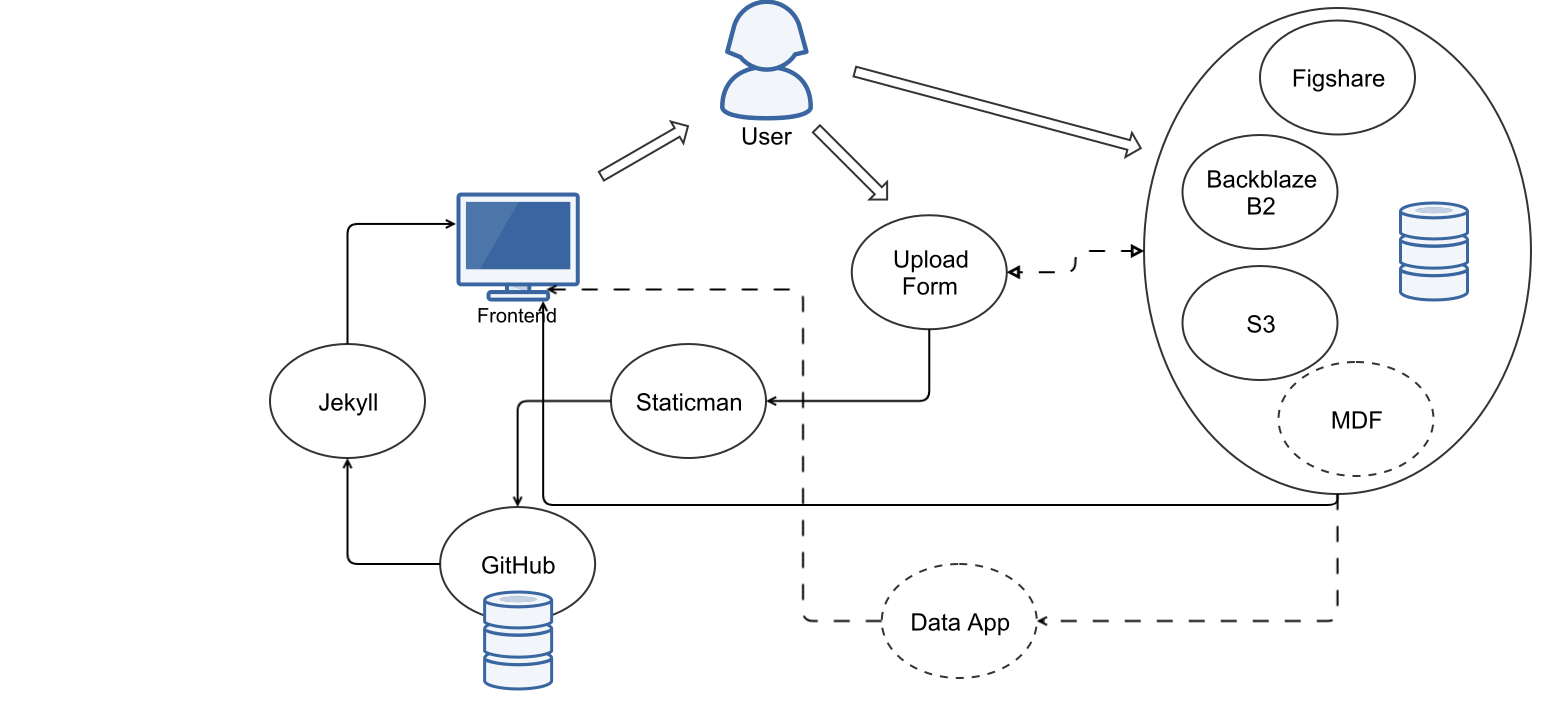
\includegraphics[width=\textwidth]{pfhub_website.png}
  \caption{Schematic overview of the PFHub framework for building
    scientific research portals, simply.}
  \centering
  \label{fig:pfhub_website}
\end{figure}

\section*{Quality control}

The framework has a fully automated test recipe deployed on Travis CI
with an environment built using the Nix Package Manager~\cite{nix}. A
fully automated test environment using continuous integration allows
all developers and users to have common feedback on code updates and
determine the compatibility of result uploads with the deployed
website. The environment is pinned to a specific version of the
Nixpkgs repository ensuring fully reproducible build and test phases
as well as ensuring that the development and automated testing
environments are identical. The full test recipe is outlined in a
\texttt{.travis.yml} file stored in the repository~\cite{travisyml}
and consists of the following steps.

\begin{itemize}
  \item Build the Nix environment from a cached storage reducing the
    build time.
  \item Run automated tests on Jupyter Notebooks using
    NBval~\cite{nbval} and Py.test~\cite{pytest}.
  \item Run validation tests on HTML files using
    HTMLProofer~\cite{htmlproofer}.
  \item Lint and test front-end Coffeescript using appropriate tools.
  \item Display a temporary version of the website using
    Surge~\cite{surge} for visual review.
\end{itemize}

\section*{(2) Availability}
\vspace{0.5cm}
\section*{Operating system}

The PFHub framework can be deployed on any platform supporting Nix,
which includes all contemporary Linux and Mac OS X platforms. Since
the framework is built with Jekyll and automated front-end processing,
it can be deployed on GitHub's Pages infrastructure, which enables
streamlined deployment without the need for any back-end
infrastructure and, thus, largely platform independent. For
development purposes, a Nix installation is required or use of the
supplied Docker container if using Windows.

\section*{Programming language}

PFHub is currently built and tested using the programming languages
and versions outlined in Table~\ref{tab:versions}.

\begin{table}[h!]
  \centering
  \caption{PFHub programming languages and corresponding supported
    versions.}
  \begin{tabular}{|l|l|}
    \hline
    Language         & Version \\
    \hline
    HTML             & 5       \\
    Jupyter Notebook & 5.4.0   \\
    JavaScript       & 5       \\
    Nix              & 2.1.3   \\
    CoffeeScript     & 1.12.7  \\
    CSS              & 4       \\
    \hline
  \end{tabular}
  \label{tab:versions}
\end{table}


\section*{Additional system requirements}

There are no additional system requirements.

\section*{Dependencies}

The entire environment can be built using the Nix Package Manager so
the only required dependency is a functional Nix installation. The
PFHub framework has over 2000 separate package dependencies using
data from the Nix package manager. The full dependency graph for PFHub
can be seen online~\cite{dependencies}.

\section*{List of contributors}

This list is for contributors to the code base, but not those that
have only uploaded output results to the website.

1. Wheeler, Daniel; A, \githublink{wd15} \\
2. Keller, Trevor; A, \githublink{tkphd} \\
3. DeWitt, Stephen J.; E, \githublink{stvdwtt} \\
4. Jokisaari, Andrea M.; D, \githublink{amjokisaari} \\
5. Schwen, Daniel; D, \githublink{dschwen} \\
6. Guyer, Jonathan E.; A, \githublink{guyer} \\

Also, see the contributors list on GitHub~\cite{contributors}.

\section*{Software location:}

{\bf Archive}

\begin{description}[noitemsep,topsep=0pt]
	\item[Name:] Zenodo
	\item[Persistent identifier:]
          \href{https://dx.doi.org/10.5281/zenodo.2592705}{10.5281/zenodo.2592705}
	\item[Licence:] NIST Software License~\cite{nistlicense}
	\item[Publisher:]  Daniel Wheeler
	\item[Version published:] v0.1
	\item[Date published:] 13/03/19
\end{description}

{\bf Code repository}

\begin{description}[noitemsep,topsep=0pt]
	\item[Name:] GitHub
	\item[Persistent identifier:] \url{https://github.com/usnistgov/pfhub/tree/v0.1}
	\item[Licence:] NIST Software License~\cite{nistlicense}
	\item[Date published:] 13/03/19
\end{description}

\section*{Languages}

English

\section*{(3) Reuse potential}

The PFHub framework can be readily adopted by other communities that
want to follow a CMS-free philosophy and use well supported external
services. The website infrastructure can be cloned as a Git repository
or downloaded as a ZIP archive and deployed with minimum effort. The
mechanism for uploading data using Staticman can be easily configured
for a new repository location. However, customizing the content of the
website for a particular scientific community would require
considerable effort. The following steps are the more challenging
aspects of deploying the framework for a new community.

\begin{itemize}
  \item Upload new data upload specifications (\emph{e.g.} the
    phase-field benchmarks in the PFHub website~\cite{pfhub}) in a
    format that Jekyll can parse, \emph{e.g.}, Jupyter Notebook,
    Markdown or HTML.
  \item Edit the \texttt{benchmarks.yaml} file to reflect the new
    upload requirements and describe the figures that need to be
    generated on the upload comparison pages.
  \item Edit the \texttt{\_config.yml} file to update links and text
    related to the configuration for all aspects of the website.
  \item Update Markdown files to reflect the new content and mission
    of the scientific community.
  \item Remove data and files that are not required by the new
    community.
\end{itemize}

Currently, a deployment for a new community has not been attempted
and, thus, the above steps need to be refined and documented.

\section*{Acknowledgments}

We gratefully acknowledge input and guidance from all participants in
the series of Phase-Field workshops held between 2015 and 2018 at the
Center for Hierarchical Material Design~\cite{workshops}.

\section*{Funding statement}

D.W. wishes to acknowledge the Materials Genome Initiative funding
allocated to the National Institute of Standards and Technology. S.J.D
wishes to acknowledge funding from the U.S. Department of Energy,
Office of Basic Energy Sciences, Division of Materials Sciences and
Engineering under Award \#DE-SC0008637 as part of the Center for
PRedictive Integrated Structural Materials Science (PRISMS Center) at
University of Michigan. PWV is grateful for the financial assistance
under the award 70NANB14H012 from the National Institute of Standards
and Technology as part of the Center for Hierarchical Materials Design
(CHiMaD).

\section*{Competing interests}

The authors declare that they have no competing interests.

\printbibliography

\end{document}
